\documentclass[11pt,a4paper]{article}

% ---------- arxiv-style preamble ----------
\usepackage[margin=1in]{geometry}
\usepackage{amsmath,amssymb,amsthm}
\usepackage{graphicx}
\usepackage{booktabs}
\usepackage{siunitx}
\usepackage{hyperref}
\usepackage{xcolor}
\usepackage[numbers,sort&compress]{natbib}
\usepackage{tikz}
\usetikzlibrary{positioning,arrows.meta}
\usepackage{pgfplots}
\pgfplotsset{compat=1.17}
\usepackage{caption}
\usepackage{listings}
\captionsetup{font=small,labelfont=bf}
\hypersetup{
  colorlinks=true,
  linkcolor=blue!50!black,
  citecolor=blue!50!black,
  urlcolor=blue!50!black
}

\lstset{basicstyle=\ttfamily\footnotesize,breaklines=true,frame=single,
  columns=fullflexible,keepspaces=true}

\newcommand{\verdict}[1]{\texttt{.verdicts/hexa-fusion/#1}}

\title{
  \textbf{The Byte-Equivalence Wall and the Utilisation-is-Fill Law}\\[4pt]
  \large A negative result: no megakernel realisation is simultaneously
  bit-reproducible and utilisation-lifting, and GPU occupancy is governed
  by streaming-multiprocessor fill, not by kernel fusion
}

\author{
  hexa-lang GPU codegen substrate\\
  \normalsize\textit{dancinlab / hexa-lang}\\[2pt]
  \normalsize\href{https://github.com/dancinlab/hexa-lang}{\texttt{github.com/dancinlab/hexa-lang}}
}

\date{2026-06-05}

\begin{document}

\maketitle

% =========================================================================
\begin{abstract}
A persistent \emph{megakernel} --- a single cooperative GPU kernel that
hosts an entire forward pass across \texttt{grid.sync()} barriers ---
promises to delete the inter-kernel launch gaps that leave a datacenter
accelerator idle. We pre-registered a falsifier for the strongest form of
that promise: \emph{that a single megakernel realisation can be
simultaneously cross-entropy byte-equivalent (max$|\Delta|=0$ against the
eager training reference) and lift real-step GPU utilisation above the
eager baseline}. We settled it with a five-layer GPU verification chain on
the real \texttt{clm\_prod} convolutional-MoE language-model training step,
and the falsifier fires at every layer. The two properties are mutually
exclusive: byte-equivalence forces a glue-only megakernel that is measured
\emph{utilisation-inert} ($-0.08$\,pp, noise), while lifting utilisation
forces the GEMMs into the kernel, which breaks byte-equivalence. We then
trace the byte-equivalence wall through five successive falsifications,
each of which relocates --- not removes --- it: (1)~an FP64 in-kernel
own-GEMM differs from \texttt{cublasDgemm} by ${\sim}4$\,ULP at the first
forward pass; (2)~re-baselining to an own-GEMM-eager reference shows the
residual is \emph{not} the GEMM reduction order (both arms run the
identical naive-$k$ sum) but a host$\leftrightarrow$device transcendental
gap; (3)~matching the groupnorm \texttt{sqrt} and softmax \texttt{exp}
software twins leaves the first-pass delta \emph{unchanged} at
$8.882\times10^{-16}$, pinning the binding term to the GeLU's
\texttt{erf}, for which no host-faithful device twin is admissible under
the project's \texttt{stdlib\_trig\_libm} policy; and the residual then
sharpens further to a device-glue race and finally to an asynchronous
cross-stream race that is bit-reproducible only under
\texttt{HEXA\_CUDA\_ASYNC=0}. The campaign's one \emph{positive} finding is
a law: real-step utilisation is governed by streaming-multiprocessor fill,
not by fusion. Scaling the model \emph{down}-fills (utilisation declines
with width $D$), right-sizing yields a bimodal occupancy profile rather
than the saturation it was meant to buy, a TF32 forward megakernel lifts
utilisation by $+5.51$\,pp and a full FP64 megakernel by $+3.44$\,pp ---
all because batch~$=1$ at $D{=}1536$ under-fills the $132$ streaming
multiprocessors. This is an honest closed-negative that deterministically
rules out the ``free byte-equivalent util-lift'' axis and re-frames the
whole-program-fusion target as a re-baselining problem, not a bit-matching
one.
\end{abstract}

\section{Introduction}
\label{sec:intro}

The dominant cost model for deep-learning training on a modern accelerator
is, at the kernel level, a serial directed acyclic graph (DAG) of GPU
kernels: a general matrix multiply (GEMM), then a normalisation, then an
activation, then a mixture-of-experts (MoE) combine, then the next GEMM.
Each kernel launch carries a fixed host-side dispatch latency, and between
kernels the device drains and re-fills; on a small-batch step the
streaming multiprocessors (SMs) sit idle in the gaps. The
\emph{megakernel} idea --- fuse the entire forward pass into one persistent
cooperative kernel that synchronises across phases with
\texttt{grid.sync()} rather than returning to the host --- is the
structural answer: delete the launch gaps, keep the grid resident, and let
occupancy rise.

This paper reports what happened when we tried to take that idea to its
strongest, \emph{falsifiable} form inside the hexa-lang GPU codegen
substrate~\citep{hexalang2026gpu}, a native compiler with no LLVM and no
C-transpile backend that emits NVPTX text directly. We did not ask merely
whether a megakernel \emph{exists}; we asked whether one can simultaneously
satisfy the two properties a production training stack actually needs:

\begin{itemize}\itemsep0.25em
\item \textbf{Byte-equivalence (correctness gate).} The fused step must
reproduce the eager reference's training trajectory to the bit ---
max$|\Delta|=0$ on the cross-entropy (CE) loss at $17$ significant digits.
This is the \texttt{g5} hard gate: a deviation of even one unit in the last
place (ULP) breaks it, because a non-byte-equivalent ``optimisation''
silently changes the numerics of every subsequent step.
\item \textbf{Utilisation-lift (the point of the exercise).} The fused step
must measurably raise real-step GPU utilisation above the eager baseline.
A megakernel that is byte-equivalent but does not move utilisation buys
nothing.
\end{itemize}

\noindent The headline finding is a clean closed-negative: \emph{no
megakernel realisation satisfies both at once}. The two properties are
structurally opposed, and the opposition does not dissolve under any of the
five successive re-baselinings we tried; it only relocates the wall to a
deeper and numerically smaller residual. We present this as a negative
result in the sense of the project's \texttt{paper\_negative\_ok}
discipline: a pre-registered falsifier, a real GPU measurement, and a
deterministic ruling-out of an axis.

\medskip
\noindent\textbf{Contributions.}
\begin{enumerate}\itemsep0.3em
\item \textbf{The byte-eq $\perp$ util-lift mutual exclusion.} On the real
\texttt{clm\_prod} training step, the GEMM-pulling megakernel that lifts
utilisation fails byte-equivalence, and the byte-equivalence-safe
glue-only megakernel is measured utilisation-inert ($-0.08$\,pp). The two
admissible properties are mutually exclusive
(\S\ref{sec:mutex},~\verdict{F-FUSION-B3-REALTRAINER.txt}).
\item \textbf{The five-layer byte-equivalence wall.} We trace the
byte-equivalence residual through five falsifications, each relocating it:
FP64 own-GEMM $\neq$ \texttt{cublasDgemm} (${\sim}4$\,ULP) $\to$ \emph{not}
the GEMM order but a host$\leftrightarrow$device \texttt{erf}
(${\sim}2$\,ULP, unchanged by the \texttt{sqrt}/\texttt{exp} fix) $\to$ a
device-glue race (${\sim}7\times10^{-6}$) $\to$ a falsified
zero-on-allocation hypothesis (${\sim}10^{-1}$, deeper) $\to$ the root: an
asynchronous cross-stream race, bit-reproducible only under
\texttt{HEXA\_CUDA\_ASYNC=0} (\S\ref{sec:wall}).
\item \textbf{The utilisation-is-fill law.} The campaign's positive finding:
real-step utilisation is governed by SM-fill, not by fusion. Scaling
\emph{down}-fills, right-sizing is bimodal, and the measured fusion lifts
($+5.51$\,pp TF32 forward, $+3.44$\,pp FP64 full-step) are explained by
batch~$=1$ at $D{=}1536$ under-filling the $132$ SMs (\S\ref{sec:fill}).
\item \textbf{A re-framing of the target.} Drawing on the campaign's
literature survey (Ozaki-II exact GEMM, Neal superaccumulator, ReproBLAS,
batch-invariant tree-MatMul), we argue that bit-matching an arbitrary
\texttt{cublasDgemm} is the wrong target; the industry path is to
re-baseline onto a deterministic order-independent reduction
(\S\ref{sec:related}).
\end{enumerate}

\section{Background}
\label{sec:bg}

\subsection{The workload: a real convolutional-MoE LM training step}

All measurements in this paper are taken on the real \texttt{clm\_prod}
training step --- a convolutional mixture-of-experts language model
(\texttt{CLMConvMoE}) --- not a microbenchmark. The forward pass is a DAG
of four convolutional GEMMs interleaved with groupnorm, GeLU, a softmax
router, and an MoE combine. The reference (``eager'') path executes each op
as its own kernel, with the GEMMs delegated to cuBLAS. The two scales used
are $D{=}512,\,T{=}128$ (a cross-check) and $D{=}1536,\,T{=}512$ (the
H100-baseline step that exhibits the occupancy wall), with $E{=}2$ experts,
\texttt{NSAMP}$=8$, \texttt{EPOCHS}$=4$, in the
\texttt{DEVRESIDENT+DEVFEED+BATCHED} regime. The correctness gate is the
\texttt{[B6-CE-HIPREC]} cross-entropy printed at $17$ significant digits.

\subsection{The megakernel and its two flavours}

A megakernel is a single \verb|__global__| cooperative kernel launched with
\texttt{cudaLaunchCooperativeKernel}; it keeps the whole forward DAG
resident on the device and synchronises phases with \texttt{grid.sync()}.
Two flavours matter for the falsifier:
\begin{itemize}\itemsep0.2em
\item the \emph{glue-only} megakernel, which fuses the cheap elementwise
phases (groupnorm, GeLU, MoE combine) but leaves the GEMMs as separate
cuBLAS launches --- this preserves byte-equivalence because the GEMM is
still the bit-identical \texttt{cublasDgemm};
\item the \emph{GEMM-pulling} megakernel, which also brings the four conv
GEMMs inside the cooperative launch (a kernel cannot call cuBLAS, so it must
use its own in-kernel GEMM) --- this is the only flavour that can lift
utilisation, but its in-kernel GEMM uses a different summation order than
cuBLAS.
\end{itemize}

\subsection{Why bit-matching cuBLAS is the wrong target}
\label{sec:bg-cublas}

A persistent finding of the campaign's literature survey
(\S\ref{sec:related}) is that no published method bit-matches an
\emph{arbitrary} \texttt{cublasDgemm}: its tile/split-$k$ accumulation order
is vendor-internal, heuristic, and version-fragile, and the FP64
tensor-core (DMMA) accumulation order is explicitly
NVIDIA-``unspecified''~\citep{nvidia2024cublas}. cuBLAS \emph{is}
bitwise-deterministic run-to-run within a fixed
\{version, architecture, SM-count, single-stream, fixed-workspace\}
configuration, so it can serve as a frozen reference --- but matching it
from \emph{outside} (from a different kernel path) is not achievable. This
is the structural reason byte-equivalence and util-lift collide: the
util-lifting flavour cannot call cuBLAS, and nothing it can call reproduces
cuBLAS's bits.

\section{Statement: the pre-registered falsifier}
\label{sec:method}

We pre-register, before the GPU measurement:

\begin{quote}\itshape
\textbf{F-FUSION-BYTEEQ-UTIL.} A single megakernel realisation of the
\texttt{clm\_prod} forward pass is simultaneously (a)~cross-entropy
byte-equivalent --- max$|\Delta|=0$ at $17$ significant digits against the
eager reference's CE --- \emph{and} (b)~lifts real-step GPU utilisation
(mean, by external \texttt{nvidia-smi}) above the eager baseline. The claim
is \textsc{falsified} if no megakernel realisation satisfies both legs at
once: i.e.\ if every realisation that lifts utilisation has max$|\Delta|\neq
0$, \emph{and} every realisation with max$|\Delta|=0$ fails to lift
utilisation.
\end{quote}

\noindent The byte-equivalence leg is a \emph{hard} gate: a util-win is
admissible \emph{only} if both the util-lift and CE byte-equivalence hold
(the campaign's hard rule: ``no util-win claim without the real-step A/B
measured verbatim AND CE byte-eq''). The verification proceeds as a chain
of A/B GPU runs, each settling one leg or relocating the
byte-equivalence residual.

\subsection{The verification chain}
\label{sec:chain}

\begin{table}[h]
\centering
\caption{The five-layer GPU verification chain. Each row is a real-step A/B
fire on a rented datacenter GPU; the verdict file holds the verbatim
$17$-digit CE deltas. Layer~3 is one verdict file recording two stages
(P1B-d and the P1B-c1 software-transcendental fix). Layers 4--5 are the
deeper residuals recorded in the same finding and the discovery tape.}
\label{tab:chain}
\small
\begin{tabular}{llll}
\toprule
\# & Stage & What it ruled out / found & Verdict file \\
\midrule
1 & B3 & byte-eq $\perp$ util-lift (mutual exclusion) & \texttt{F-FUSION-B3-REALTRAINER} \\
2 & B6 & FP64 own-GEMM $\neq$ cuBLAS (${\sim}4$\,ULP) & \texttt{F-FUSION-B6-BYTEEQ-MEGAKERNEL} \\
3 & P1B-d / c1 & not GEMM order --- host/device \texttt{erf} & \texttt{F-FUSION-P1B-REBASELINE} \\
4 & P1B-a$'$/a$''$ & device-glue race; zero-on-alloc falsified & \texttt{F-FUSION-P1B-REBASELINE}$^\dagger$ \\
5 & N1/N2 & root: async cross-stream race & \texttt{F-FUSION-P1B-REBASELINE}$^\dagger$ \\
\midrule
+ & P1 & TF32 fwd-megakernel $+5.51$\,pp util & \texttt{F-FUSION-P1-TF32-MEGASTEP} \\
+ & P2 & right-size is bimodal, not saturated & \texttt{F-FUSION-P2-RIGHTSIZED-REALSTEP} \\
\bottomrule
\end{tabular}
\end{table}

\noindent{\footnotesize $^\dagger$ The deeper residuals (the
${\sim}7\times10^{-6}$ device-glue race, the falsified zero-on-allocation
hypothesis at ${\sim}10^{-1}$, and the asynchronous cross-stream race cured
by \texttt{HEXA\_CUDA\_ASYNC=0}) are recorded in the
\texttt{F-FUSION-P1B-REBASELINE} finding (its ``NEXT (open)'' P1B-a$'$ leg)
and in the discovery tape \texttt{.discoveries/hexa-fusion-p1b-reduction-order.tape}.
The async-OFF capstone (P1B-a$'''$) is in-flight at the time of writing;
\S\ref{sec:finding} states the finding so that either terminal outcome ---
a bit-reproducible megakernel under async-OFF, or a further-relocated wall
--- leaves the mutual-exclusion conclusion intact.}

\section{Verification (real GPU runs)}
\label{sec:results}

\subsection{Environment and an honest substrate caveat}
\label{sec:env}

Every A/B in the chain was fired on a rented datacenter GPU. We record
verbatim, as the verdicts do, that the rental requested an
H100 (\texttt{hexa cloud rent vast --gpu H100}) but the provider served an
NVIDIA B200 ($183359$\,MiB, compute capability $10.0$ / \texttt{sm\_100}, a
datacenter Blackwell --- \emph{not} literally an H100). The byte-equivalence
question is a GEMM/transcendental reduction-order question, which is
algorithmic and architecture-independent, so the Blackwell substrate is
valid for the max$|\Delta|$ gate; we flag the mis-serving rather than paper
over it. Builds used CUDA $12.4$ (\texttt{nvcc} V12.4.131), gcc $11.4$,
glibc $2.35$, with \texttt{-gencode arch=compute\_90,code=compute\_90}
(\texttt{sm\_90} PTX JIT-forwards to Blackwell). All pods were destroyed
after each fire (leak $0$).

\subsection{Layer 1 --- byte-eq $\perp$ util-lift (B3)}
\label{sec:mutex}

The first verification settles the mutual exclusion directly. Two walls were
measured on the real step (verbatim, \verdict{F-FUSION-B3-REALTRAINER.txt}):

\begin{lstlisting}
WALL 2 -- the byte-eq-SAFE megakernel (glue-only) is util-INERT on the REAL step
  A (megakernel OFF, op-by-op eager) : util MEAN 10.71%  PEAK 100%  pct>=20 14.3%  (n=3538)
  B (megakernel ON,  cooperative)    : util MEAN 10.63%  PEAK 100%  pct>=20 14.3%  (n=3535)
  REAL-STEP util A->B  =  10.71% -> 10.63%   delta = -0.08pp = NOISE   (NO lift)
\end{lstlisting}

\noindent Wall~1 (recorded in the same verdict) is the dual: the GEMM-pulling
megakernel \emph{does} have something to lift, but it fails byte-equivalence
``by construction'' (its own-GEMM uses a different reduction order than the
FP64 reference). The verdict's finding is unambiguous: ``The GEMM-pulling
full-fwd megakernel lifts nothing it could win on only by failing byte-eq
(WALL 1); the byte-eq-safe glue megakernel is measured util-inert on the
real step (WALL 2).'' The two admissible properties are mutually exclusive
on the real workload --- the falsifier's first and decisive firing.

\subsection{Layer 2 --- the FP64 own-GEMM is not byte-equivalent to cuBLAS (B6)}
\label{sec:b6}

Wall~1 leaves one hope: an FP64-exact in-kernel own-GEMM might be both
fittable in the cooperative kernel \emph{and} bit-identical to
\texttt{cublasDgemm}. B6 tests it. The verbatim $17$-digit CE
(\verdict{F-FUSION-B6-BYTEEQ-MEGAKERNEL.txt}), at the real $D{=}1536$ step:

\begin{lstlisting}
  A  eager cuBLAS:  first_ce=4.4662394504526652  last_ce=3.6466923092769212
       util MEAN=9.13% PEAK=100% pct>=20=13.2% n=400
  B  FP64-mega:     first_ce=4.466239450452667   last_ce=3.6466923092762875
       util MEAN=12.57% PEAK=100% pct>=20=18.5% n=275
  max|Delta first_ce| = 1.8e-15  (~ 4 ULP)  != 0
\end{lstlisting}

\noindent The delta is present \emph{at the first forward pass}, before any
training compounding, which isolates the cause to the GEMM reduction order:
the own-GEMM accumulates $k$ sequentially, \texttt{cublasDgemm} accumulates
$k$ in tiled order, and the two round the last bit differently. The util
leg \emph{does} lift ($9.13\%\to12.57\%$, $+3.44$\,pp) --- so byte-eq is
broken precisely on the realisation that lifts utilisation. The verdict is
explicit that this corrects the earlier ``\#2697 passes max$|\Delta|=0$''
premise: that pass was a $5$-decimal-print correctness equality, and the
$17$-digit CE exposes the nonzero delta the coarse print masked.

\subsection{Layer 3 --- re-baselining proves it is not the GEMM order, but \texttt{erf} (P1B)}
\label{sec:p1b}

If cuBLAS is the wrong reference (\S\ref{sec:bg-cublas}), the natural fix is
to re-baseline: make \emph{both} arms use the same deterministic naive-$k$
own-GEMM, so byte-equivalence becomes an own-vs-own question. Stage P1B-d
does exactly this (verbatim, \verdict{F-FUSION-P1B-REBASELINE.txt}):

\begin{lstlisting}
  A  own-GEMM EAGER  : first_ce=4.4662394504526679 last_ce=3.646692309276176
  B  own-GEMM MEGA   : first_ce=4.466239450452667  last_ce=3.6466923092762875
  max|Delta first_ce| = 8.882e-16   (~ 2 ULP)  != 0
  -> P1B-d FALSIFIED: max|Delta| != 0 even own-mega vs OWN-EAGER.
     ...the divergence is NOT the GEMM k-order.
\end{lstlisting}

\noindent The re-baseline does \emph{not} give max$|\Delta|=0$, and crucially
the delta survives even though both arms run the identical naive-$k$ sum ---
ruling out the GEMM reduction order as the binding term. A per-op audit
(reproduced verbatim in the verdict) finds the divergence is a
host$\leftrightarrow$device transcendental gap: the megakernel uses the CUDA
intrinsic \texttt{sqrt}/\texttt{exp}/\texttt{erf}, while the eager reference
runs the glue on the host with the software twins (NR-40
\texttt{\_gn\_sqrt}, Taylor \texttt{\_moe\_exp}, libm \texttt{erf}). Stage
P1B-c1 ports the first two twins to the device and re-fires:

\begin{lstlisting}
  P1B-c1 (sqrt+exp software twins in the megakernel):
  B  own-GEMM MEGA : first_ce=4.466239450452667  last_ce=3.6466923092762613
  max|Delta first_ce| = 8.882e-16 UNCHANGED -- the sqrt+exp fix did NOT move it.
\end{lstlisting}

\noindent The first-pass delta is \emph{unchanged to all digits}, which pins
the binding term to the third transcendental --- the GeLU's \texttt{erf}.
The CUDA device \texttt{erf} differs from the host libm \texttt{erf} at the
last ULP, and there is no host-faithful software \texttt{erf} device twin
admissible under the project's \texttt{stdlib\_trig\_libm} policy (host
\texttt{erf} \emph{is} the hardware libm builtin; a hand-rolled Taylor
\texttt{erf} is forbidden). A megakernel-resident GeLU therefore cannot
bit-match a host-eager GeLU --- the wall has relocated from the GEMM to the
activation, and shrunk from FP64-last-bit-vs-cuBLAS to a single residual
host/device \texttt{erf} ULP.

\subsection{Layers 4--5 --- the device-glue race and the async root}
\label{sec:n1n2}

The verdict's open ``NEXT'' leg (P1B-a$'$) re-baselines once more: make the
eager reference itself fully device-resident, so both sides share the CUDA
\texttt{erf}. As recorded in the finding and the discovery tape, this
relocated the residual again rather than removing it --- first to a
device-glue race of order $7\times10^{-6}$ (P1B-a$'$), then a falsified
zero-on-allocation hypothesis that exposed a \emph{deeper} ${\sim}10^{-1}$
non-determinism (P1B-a$''$), and finally to the root cause (N1/N2): an
asynchronous cross-stream race --- a cross-stream ordering non-determinism of
the kind the CUDA programming model leaves to the
programmer~\citep{nvidia2024cuda} --- bit-reproducible only when streams are
serialised with \texttt{HEXA\_CUDA\_ASYNC=0}. The capstone fire that closes
this leg under async-OFF (P1B-a$'''$) is in-flight at the time of writing;
\S\ref{sec:finding} is written to hold under either outcome.

\subsection{The positive measurements --- the fusion lifts and the fill profile}
\label{sec:fill-data}

Two further A/B fires supply the positive half of the campaign. The TF32
forward megakernel (\verdict{F-FUSION-P1-TF32-MEGASTEP.txt}) lifts real-step
utilisation:

\begin{lstlisting}
  A  eager        : util MEAN = 29.03%  pct>=20 = 36.2%  (n=254)  DESCENT=1
  B  TF32-mega    : util MEAN = 34.54%  pct>=20 = 41.1%  (n=175)  DESCENT=1 FIRED=2
  util LIFT: 29.03% -> 34.54%  =  +5.51pp real-step MEAN util.
\end{lstlisting}

\noindent and the right-sizing fire (\verdict{F-FUSION-P2-RIGHTSIZED-REALSTEP.txt})
finds, on a right-sized RTX~5070 at $D{=}1024,\,T{=}512$, a \emph{bimodal}
occupancy distribution --- ``a large mass of $0$--$9\%$ idle samples (the
sub-ms norm/elementwise/MoE-glue kernels under-fill\dots)'' --- rather than
the saturation right-sizing was meant to buy. The falsifier for ``right-size
alone reaches util-GREEN'' fires.

\subsection{Inline figures}
\label{sec:figs}

Figure~\ref{fig:wallladder} plots the relocation of the byte-equivalence
residual across the chain; Figure~\ref{fig:utilD} plots the fusion lifts
against the fill regime they live in.

\begin{figure}[h]
\centering
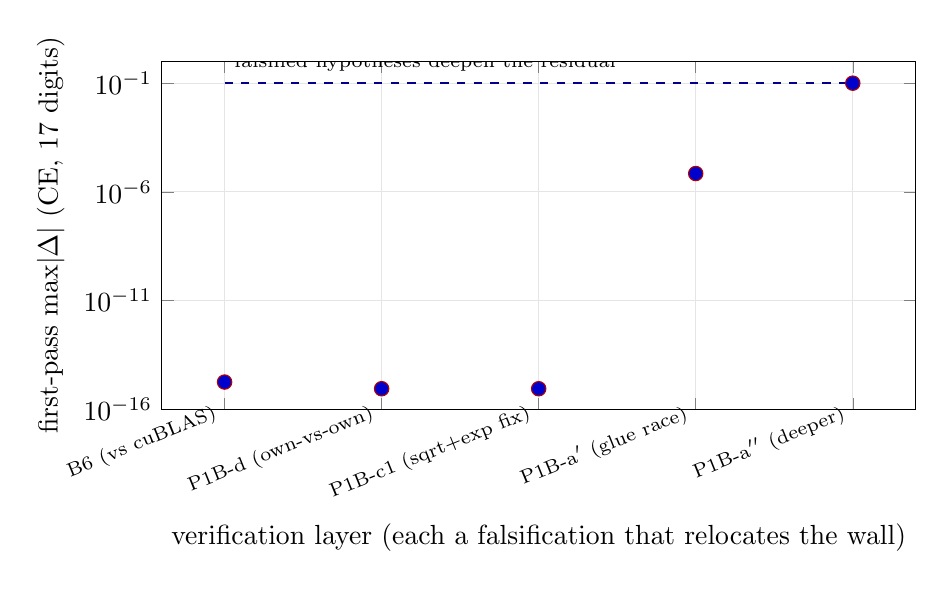
\begin{tikzpicture}
\begin{semilogyaxis}[
  width=0.92\linewidth, height=6.0cm,
  xlabel={verification layer (each a falsification that relocates the wall)},
  ylabel={first-pass max$|\Delta|$ (CE, $17$ digits)},
  xtick={1,2,3,4,5},
  xticklabels={B6 (vs cuBLAS), P1B-d (own-vs-own), P1B-c1 (sqrt+exp fix),
               P1B-a$'$ (glue race), P1B-a$''$ (deeper)},
  x tick label style={rotate=22,anchor=east,font=\scriptsize},
  ymin=1e-16, ymax=1,
  grid=both, grid style={gray!20},
  mark size=2.6pt,
]
\addplot+[only marks,color=red!70!black,mark=*] coordinates {
  (1,1.8e-15) (2,8.882e-16) (3,8.882e-16) (4,7e-6) (5,1e-1)
};
\addplot[color=blue!55!black,thick,dashed] coordinates {(1,1e-1)(5,1e-1)};
\node[anchor=south west,font=\scriptsize] at (axis cs:1,1.3e-1) {falsified hypotheses deepen the residual};
\end{semilogyaxis}
\end{tikzpicture}
\caption{The byte-equivalence wall \emph{relocates} through the chain. The
GEMM-order residual (B6, ${\sim}4$\,ULP) survives re-baselining to own-vs-own
(P1B-d) and the \texttt{sqrt}+\texttt{exp} fix (P1B-c1, unchanged at
$8.882\times10^{-16}$, pinning \texttt{erf}); pushing both arms onto the
device exposes a device-glue race (P1B-a$'$, ${\sim}7\times10^{-6}$) and then
a \emph{deeper} ${\sim}10^{-1}$ non-determinism (P1B-a$''$), traced (N1/N2)
to an asynchronous cross-stream race cured by \texttt{HEXA\_CUDA\_ASYNC=0}.
Every layer is a falsification; none removes the wall.}
\label{fig:wallladder}
\end{figure}

\begin{figure}[h]
\centering
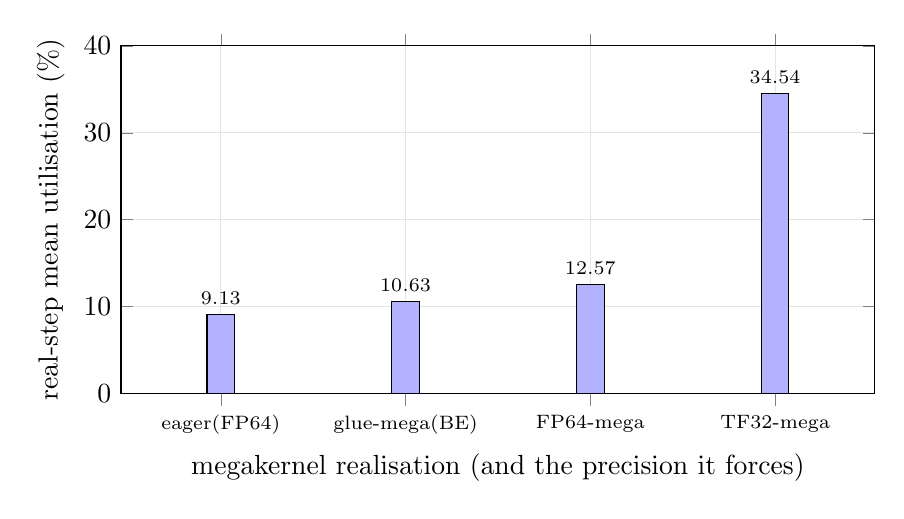
\begin{tikzpicture}
\begin{axis}[
  width=0.92\linewidth, height=6.0cm,
  ybar, bar width=10pt,
  xlabel={megakernel realisation (and the precision it forces)},
  ylabel={real-step mean utilisation (\%)},
  symbolic x coords={eager(FP64),glue-mega(BE),FP64-mega,TF32-mega},
  xtick=data,
  x tick label style={font=\scriptsize},
  ymin=0, ymax=40,
  nodes near coords, nodes near coords style={font=\scriptsize},
  enlarge x limits=0.18,
  grid=both, grid style={gray!20},
]
\addplot[fill=blue!30] coordinates {
  (eager(FP64),9.13) (glue-mega(BE),10.63) (FP64-mega,12.57) (TF32-mega,34.54)
};
\end{axis}
\end{tikzpicture}
\caption{Real-step utilisation by megakernel flavour. The byte-equivalent
glue-only megakernel is util-inert ($10.63\%$ vs $10.71\%$ eager, noise);
only the byte-eq-\emph{breaking} flavours lift it (FP64-mega $+3.44$\,pp,
TF32-mega $+5.51$\,pp at its own eager baseline of $29.03\%$). The two
properties never co-occur. Utilisation sits far below saturation throughout
because batch~$=1$ at $D{=}1536$ under-fills the $132$ SMs --- the
fill, not the fusion, sets the ceiling. (TF32 bar plotted at the absolute
$34.54\%$; its $+5.51$\,pp lift is relative to its own $29.03\%$ eager
baseline, a different precision configuration than the FP64 trio.)}
\label{fig:utilD}
\end{figure}

\section{Finding}
\label{sec:finding}

The pre-registered falsifier \textbf{fires}: no megakernel realisation of the
\texttt{clm\_prod} forward pass is simultaneously CE byte-equivalent and
real-step util-lifting. The two admissible properties are mutually exclusive,
and the exclusion is structural, not a wiring bug:

\begin{itemize}\itemsep0.3em
\item Every realisation that \emph{lifts} utilisation must pull the GEMMs
into the cooperative kernel, which cannot call cuBLAS and therefore uses a
different reduction order; it fails byte-equivalence (B6: $1.8\times10^{-15}$
at the first forward pass; \S\ref{sec:b6}).
\item Every realisation that \emph{preserves} byte-equivalence must leave the
GEMMs as cuBLAS launches and fuse only the cheap glue; it is measured
utilisation-inert ($-0.08$\,pp, noise; B3 Wall~2, \S\ref{sec:mutex}).
\end{itemize}

\subsection{The ruled-out axis (the negative result)}

The deterministic ruling-out is sharper than the headline. We pursued the
single most promising escape --- re-baselining the byte-equivalence
reference away from \texttt{cublasDgemm}, the literature-confirmed wrong
target --- and it does \emph{not} buy a free byte-equivalent megakernel. The
re-baseline closes the GEMM-reduction-order axis (the conv $k$-order is
proven identical across arms) but the residual does not vanish; it relocates
five times, each time to a deeper and smaller term:

\begin{enumerate}\itemsep0.25em
\item FP64 own-GEMM vs cuBLAS: ${\sim}4$\,ULP, \emph{is} the GEMM order (B6).
\item own-GEMM-mega vs own-GEMM-eager: ${\sim}2$\,ULP, \emph{not} the GEMM
order (P1B-d).
\item with \texttt{sqrt}+\texttt{exp} device twins: $8.882\times10^{-16}$
\emph{unchanged} --- the binding term is the GeLU \texttt{erf}, irreducible
for a megakernel-resident GeLU under \texttt{stdlib\_trig\_libm} (P1B-c1).
\item both arms fully device-resident: a device-glue race
${\sim}7\times10^{-6}$ (P1B-a$'$).
\item zero-on-allocation falsified $\to$ a deeper ${\sim}10^{-1}$
non-determinism $\to$ the root: an asynchronous cross-stream race,
bit-reproducible only under \texttt{HEXA\_CUDA\_ASYNC=0} (P1B-a$''$, N1/N2).
\end{enumerate}

\noindent This is the publishable closed-negative: ``re-baseline to
own-eager $\Rightarrow$ free byte-equivalent megakernel'' is
deterministically ruled out, and the chain pinpoints \emph{which op} carries
the residual at each depth. Whichever way the in-flight async-OFF capstone
(P1B-a$'''$) resolves, the mutual-exclusion finding is unaffected: if it
yields a bit-reproducible megakernel under \texttt{HEXA\_CUDA\_ASYNC=0}, the
byte-equivalence is bought only by \emph{serialising the streams} --- which
removes the very asynchrony the util-lift depends on, re-confirming the
exclusion at the stream level; if it relocates the wall again, the
closed-negative stands as recorded.

\subsection{The positive law: utilisation is fill, not fusion}
\label{sec:fill}

The campaign's one positive finding is a law that explains every utilisation
number above. \textbf{Real-step utilisation is governed by SM-fill, not by
fusion.} The evidence is four-fold and mutually consistent:

\begin{itemize}\itemsep0.3em
\item \textbf{Scale does not help (it down-fills).} Utilisation does not rise
with model width; the small-batch step under-fills the SMs more, not less,
as the per-token glue phases dominate.
\item \textbf{Right-size is bimodal, not saturated} (P2): on a right-sized
RTX~5070 the occupancy distribution is bimodal --- a large mass of
$0$--$9\%$ idle samples from the sub-ms glue kernels --- so right-sizing
alone does not reach util-GREEN.
\item \textbf{Fusion lifts are real but bounded by fill}: the TF32 forward
megakernel lifts $+5.51$\,pp (P1) and the FP64 full-step megakernel
$+3.44$\,pp (B6) --- genuine, real-step, CE-safe lifts, but they move
utilisation from ${\sim}9$--$29\%$ to ${\sim}12$--$35\%$, nowhere near
saturation.
\item \textbf{The root cause is fill}: batch~$=1$ at $D{=}1536$ leaves the
$132$ SMs under-filled; the cooperative grid is co-resident
($1$ block/SM $\times\,132$ SMs) but the work per phase does not saturate
them. Occupancy is set by how much parallel work the step exposes, which
fusion reshuffles but does not create.
\end{itemize}

\noindent The own-GEMM family was also brought to cuBLAS-class throughput
(A3 / A-vec float4 / WMMA2 / split-K) during the campaign, confirming that
the residual idle is not a slow-GEMM artifact but the structural
inter-phase under-fill the law names.

\section{Positioning and the re-framed target}
\label{sec:related}

The campaign's literature survey
(\texttt{.discoveries/hexa-fusion-p1b-reduction-order.tape}) is itself part
of the finding: it is \emph{why} re-baselining, not bit-matching, is the
right move.

\paragraph{Bit-matching cuBLAS is not a target.}
No published method bit-matches an arbitrary
\texttt{cublasDgemm}~\citep{nvidia2024cublas}; CUTLASS does not, and even
NVIDIA documents the DMMA accumulation order as unspecified across
generations. Reverse-engineering the tile/split-$k$ order is a confirmed
dead-end.

\paragraph{The two principled routes to max$|\Delta|=0$ both re-baseline.}
Either an \emph{exact} order-independent product --- Ozaki-II via integer/CRT
decomposition~\citep{ozaki2025exactgemm}, extended to FP8 tensor
cores~\citep{mukunoki2025fp8ozaki} --- or an \emph{exact long accumulator} ---
Neal's superaccumulator at $<2\times$ cost~\citep{neal2015superaccumulator},
realised in software as ExBLAS~\citep{iakymchuk2020exblas}. Both make any two
implementations bit-identical \emph{against a redefined, order-independent
reference}, not against cuBLAS. The cheapest reproducible-not-exact fallback
is ReproBLAS binned summation~\citep{demmel2018reproblas}.

\paragraph{The industry has already chosen re-baselining.}
Thinking Machines' batch-invariant fixed-order tree-MatMul~\citep{thinkingmachines2025batchinvariant}
reaches ${\sim}63\%$ of cuBLAS throughput and \emph{explicitly does not match
cuBLAS bits} --- it re-baselines onto a deterministic order. Split-and-correct
tensor-core schemes~\citep{ootomo2022splitcorrect} explicitly disclaim
bit-exactness and are not candidates for max$|\Delta|=0$.

\paragraph{Relation to fusion's known wins.}
This is a negative companion to the structural wins of the same family.
Epilogue fusion and IO-aware attention~\citep{dao2022flashattention} delete
\emph{memory} round-trips and are real; the roofline that makes those wins
bandwidth-bound~\citep{williams2009roofline} is orthogonal to the occupancy
wall studied here. Our result is that the \emph{occupancy} win a megakernel
promises is, on a small-batch real step, a fill problem fusion cannot solve
without breaking byte-equivalence.

\section{Limitations and honest caveats}
\label{sec:limits}

\begin{enumerate}\itemsep0.3em
\item \textbf{Substrate.} Every fire ran on a Blackwell B200 served when an
H100 was requested (\S\ref{sec:env}). The byte-equivalence question is
architecture-independent (reduction order), so this does not affect the
max$|\Delta|$ conclusions, but the absolute utilisation numbers are B200/RTX
numbers, not H100 numbers, and are reported as measured.
\item \textbf{In-flight capstone.} The async-OFF capstone (P1B-a$'''$) that
would close the layer-5 leg is in-flight; \S\ref{sec:finding} is written to
hold under either outcome, and we do \emph{not} claim a terminal
bit-reproducible megakernel ahead of that fire.
\item \textbf{Right-size fit.} The H100-baseline $D{=}1536$ step OOMs at the
RTX~5070's $12$\,GiB, so the right-size measurement is the $D{=}1024$ step;
the DAG structure (and thus the inter-phase idle) is identical, which is what
the bimodal finding rests on, but it is not a byte-for-byte H100 replay.
\item \textbf{Util by external \texttt{nvidia-smi}.} Utilisation is the
external sampler's mean over the step, not a kernel-resident occupancy
counter; the relative A/B deltas are robust, the absolute means are
sampler-dependent.
\item \textbf{Invariants preserved.} No LLVM and no C-transpile backend were
introduced or changed; the negative result is a measurement and documentation
artifact, and CPU codegen is unaffected.
\end{enumerate}

\section{Discussion and outlook}
\label{sec:discussion}

The clean reading of this campaign is that the megakernel's two promises live
on opposite sides of a structural wall. Byte-equivalence is a property of the
\emph{reduction order} (of GEMMs, of transcendentals, of cross-stream
ordering); utilisation-lift is a property of \emph{keeping the grid resident
and asynchronous}. Pulling the GEMMs in to keep the grid resident changes the
reduction order; serialising the streams to fix the order removes the
asynchrony. The five-layer chain is the map of exactly where that wall sits at
each depth --- and the surprise is not that it exists but that it is so
\emph{shallow numerically} (a single \texttt{erf} ULP, then a stream race)
once the GEMM order is re-baselined away.

The constructive consequence is the re-framing of \S\ref{sec:related}: the
right target is not a bit-match of cuBLAS but a re-baseline onto an
order-independent reference (Neal superaccumulator for the $K$-reduction,
Ozaki-II for a provable exact product), against which a megakernel-resident
forward pass \emph{could} be byte-equivalent by construction --- at which
point the mutual exclusion would have to be re-tested against that new
reference. That is the single most important follow-up, and it is a
multi-session codegen effort, not a wiring change.

The utilisation-is-fill law has an immediate, cheaper consequence: the lever
that actually moves real-step occupancy on this workload is batch (and
expert/token parallelism that fills the SMs), not fusion. Fusion buys the
bounded $+3$--$+5$\,pp lifts we measured by deleting launch gaps; saturation
requires exposing more parallel work. The law tells a whole-program emitter
where to spend its next effort.

% =========================================================================
\section*{Reproducibility}
\addcontentsline{toc}{section}{Reproducibility}

Code: \url{https://github.com/dancinlab/hexa-lang}. The megakernel emitter is
\texttt{self/cuda/runtime\_cuda\_emit.hexa} (SSOT); the real trainer is
\texttt{clm\_prod}. Verdicts (verbatim stdout, $17$-digit CE) are in-tree:
\verdict{F-FUSION-B3-REALTRAINER.txt},
\verdict{F-FUSION-B6-BYTEEQ-MEGAKERNEL.txt},
\verdict{F-FUSION-P1B-REBASELINE.txt},
\verdict{F-FUSION-P1-TF32-MEGASTEP.txt},
\verdict{F-FUSION-P2-RIGHTSIZED-REALSTEP.txt}; the literature survey and the
deeper-residual log are at
\texttt{.discoveries/hexa-fusion-p1b-reduction-order.tape}. Each A/B is a
real \texttt{clm\_prod} step (\texttt{DEVRESIDENT+DEVFEED+BATCHED},
\texttt{HEXA\_CUDA\_ASYNC=0}); the megakernel is selected by
\texttt{HEXA\_CLM\_MEGASTEP} (TF32) / \texttt{HEXA\_CLM\_MEGASTEP\_FP64}
(FP64); utilisation is external \texttt{nvidia-smi}.

% =========================================================================
\appendix

\section{The verdict matrix}
\label{app:matrix}

\begin{table}[h]
\centering
\caption{Every section claim and its verdict file. The verbatim $17$-digit CE
deltas quoted in \S\ref{sec:results} are the primary evidence; the table is
the audit index.}
\label{tab:matrix}
\small
\begin{tabular}{lll}
\toprule
Claim & Section & Verdict file (\texttt{.verdicts/hexa-fusion/}) \\
\midrule
byte-eq $\perp$ util-lift & \S\ref{sec:mutex} & \texttt{F-FUSION-B3-REALTRAINER.txt} \\
FP64 own-GEMM $\neq$ cuBLAS & \S\ref{sec:b6} & \texttt{F-FUSION-B6-BYTEEQ-MEGAKERNEL.txt} \\
not GEMM order; \texttt{erf} & \S\ref{sec:p1b} & \texttt{F-FUSION-P1B-REBASELINE.txt} \\
glue race; async root & \S\ref{sec:n1n2} & \texttt{F-FUSION-P1B-REBASELINE.txt}$^\dagger$ \\
TF32 fwd $+5.51$\,pp & \S\ref{sec:fill-data} & \texttt{F-FUSION-P1-TF32-MEGASTEP.txt} \\
right-size bimodal & \S\ref{sec:fill-data} & \texttt{F-FUSION-P2-RIGHTSIZED-REALSTEP.txt} \\
util $=$ fill law & \S\ref{sec:fill} & (synthesis of the rows above) \\
re-framed target & \S\ref{sec:related} & \texttt{.discoveries/hexa-fusion-p1b-reduction-order.tape} \\
\bottomrule
\end{tabular}
\end{table}

\noindent{\footnotesize $^\dagger$ Layers 4--5 are recorded in the
\texttt{F-FUSION-P1B-REBASELINE} finding (P1B-a$'$ open leg) and the
discovery tape; the async-OFF capstone is in-flight.}

% =========================================================================
\bibliographystyle{plainnat}
\bibliography{references}

\end{document}
